%----------------------------------------------------------------------
\section{Formalization of Quantum Error Correction}\label{sec:QECBackground}
%----------------------------------------------------------------------

\begin{figure}[!b]
    \centering
    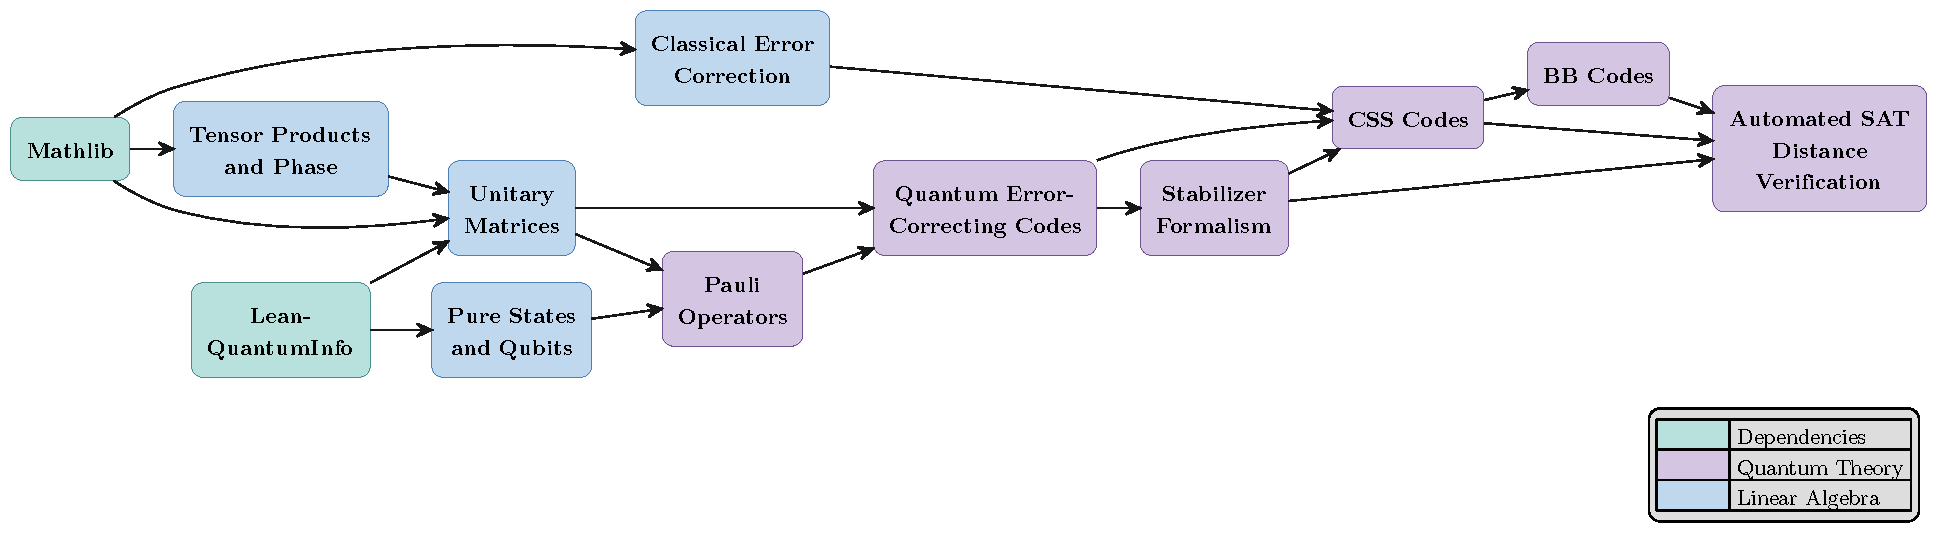
\includegraphics[width=\linewidth]{Figures/fig3_theory_map.pdf}
    \caption{Map of the formalized quantum-error-correction stack. Arrows are
    machine-checked correspondence theorems; the rightmost layer feeds into the
    SAT-based distance pipeline of \Cref{sec:smt}.}
    \label{fig:qmap}
\end{figure}

% To demonstrate the interesting challenges faced in formalizing Quantum Error
% Correction and compare writing in Lean to informal mathematical writing, we
% will present background and formalization simultaneously. In \ref{fig:qmap},
% we map the major accomplishments of the theory and how they relate to each
% other. The major accomplishments of the repository are the theorems proved
% relating the distance of Quantum Error-Correcting Codes to the linear
% algebraic and boolean versions of the statements, and most parts of the
% repository are leading towards those results.
%

This section builds the stack from \Cref{fig:qmap} bottom-up: qubit states,
$n$-qubit unitaries, the Pauli group with phases, the binary symplectic
representation, abstract QEC codes, stabilizer codes, and finally the CSS and
Bivariate Bicycle families. For each layer we describe the formalization choice,
the machine-checked correspondence to the layer below, and the type-theoretic
friction that distinguishes the Lean development from a pen-and-paper account.
The chain of correspondences ending at the binary symplectic matrix is what
makes the SAT-based distance pipeline of \Cref{sec:smt} end-to-end: a distance
bound discharged at the bottom transports, by a Lean theorem, to a bound on the
quantum code at the top.

\subsection{Qubit States}
\label{sec:qc}

% We begin with our formalization of quantum states.
% Formalization of quantum algorithms have been studied by the SQIR line of
% literature \cite{hietala2021} as well as CoqQ \cite{coqq}.
% Unfortunately, as they are formalized using a different proof assistant,
% we do not have an easy way to make use of them.
% On the other hand, the Lean-QuantumInfo \cite{leanquantuminfo} project does
% not specialize its quantum states to the qubit space, so this is where our
% formalization starts.
%
% When we are asked to define a $n$-qubit state, the first answer is perhaps a
% $2^n$-dimensional vector over $\bbC$.
% On the other hand, when we are asked to write down the general form of a
% quantum state $\ket{\psi}$, we often write the expression
% $$\ket{\psi}=\sum_{x\in\set{0, 1}^n}\alpha_x\ket{x}.$$
% Now, the $n$-qubit standard basis, indexed using $n$-bit binary strings, is
% certainly isomorphic to the space $\bbC^{2^n}$, simply by collecting all the
% amplitudes $\alpha_x$.
% This syntactic mismatch, and equivalence up to isomorphism, however, represent
% a design decision that we must make through our proof engineering.
%
% In Lean, vectors of the form $\mathbb{F}^n$ are conventionally formalized
% using the property
% \begin{equation}
%     \label{eq:vec-equiv-fn}
%     \mathbb{F}^n\cong \Fun(\bbN_n, \mathbb{F})
% \end{equation}
% where $\bbN_n=\set{0, 1, \ldots, n-1}$ denotes the set of natural numbers up
% to $n$.
% Perhaps this is unsurprising, since $Y^X$ is the standard notation for the set
% of functions $\Fun(X, Y)$ in many mathematics communities.
% We follow the same conventions and formalize our quantum state by
% $\Fun(\set{0, 1}^n, \bbC)$
% up to the usual amplitude normalization constraints;
% that is, we would write $\mathbb{C}^{\set{0, 1}^n}$, instead of
% $\mathbb{C}^{2^n}$ like in other verified frameworks such as SQIR.
% One benefit of our formalism is that it allows us to treat tensor products
% more naturally.
% For example, suppose we have two standard basis states, $\ket{101}$ and
% $\ket{001}$.
% To combine them then, we would write
% $$\ket{101}\otimes\ket{001}=\ket{101001},$$
% simply concatenating the two strings together.
% On the other hand, in formalizations using $2^n$-dimensional vectors instead,
% taking the product between qubit states would involve bit-shifting the
% operands, which may be more tedious to analyze.
%

The SQIR development~\cite{hietala2021} and CoqQ~\cite{coqq} formalize quantum
states in Rocq Prover, and the Lean-QuantumInfo project~\cite{leanquantuminfo}
formalizes general finite-dimensional quantum states in Lean. None of these
specialize the state space to qubits in the way we need, so we start the stack
ourselves.

\paragraph{Choice of index set.} A textbook quantum researcher writes a pure
state as
$\ket{\psi} = \sum_{x \in \{0,1\}^n} \alpha_x \ket{x}$,
i.e.\ as an assignment of amplitudes to bit strings. A textbook formalizer
writes it as an element of $\mathbb{C}^{2^n}$. The two views are isomorphic, but
Lean represents a finite-dimensional vector by its function form
\begin{equation}
    \label{eq:vec-equiv-fn}
    \mathbb{F}^n \cong \Fun(\bbN_n, \mathbb{F}), \qquad \bbN_n = \{0, 1, \ldots, n-1\},
\end{equation}
and the choice of index set is a load-bearing design decision: every later
definition is parametrized by it. We diverge from SQIR's $\mathbb{C}^{2^n}$
convention and adopt $\Fun(\{0,1\}^n, \mathbb{C})$, written
$\mathbb{C}^{\{0,1\}^n}$ with the usual normalization. The payoff is that
tensor products on basis states become string concatenation, $\ket{101} \otimes
\ket{001} = \ket{101001}$, instead of an arithmetic identity on bit-shifts; this
matters because Pauli operators are most naturally indexed by which qubit they
act on, not by a position in a flattened $2^n$-array.

\subsection{Quantum Operators}

% There are many sophisticate and powerful formalizations of quantum operations.
% These existing frameworks have had to face many challenges, type-theoretic and
% otherwise, in order to describe circuit-like constructions:
% for example, to add a two-qubit gate on the $i$-th and $j$-th qubits in an
% $n$-qubit system.
% For our purpose of studying quantum error correction,
% we will avoid re-inventing those wheels, and leave fleshing out such a
% framework in Lean for future work.
% For quantum error corrections, it would suffice if we can ``glue'' states and
% operators together consistently.
% In particular, we have to verify that for all states $\ket{\phi_1}$ and
% $\ket{\phi_2}$, and all operators $U_1$ and $U_2$,
% we have
% \begin{equation}
% \label{eq:kron-ustate}
% (U_1\otimes U_2)(\ket{\phi_1}\otimes\ket{\phi_2})=U_1\ket{\phi_1}\otimes
% U_2\ket{\phi_2}.
% \end{equation}
%
% As simple as \Cref{eq:kron-ustate} may seem,
% there is already a gap that we must address carefully.
% Colloquially, we often use the term \emph{tensor product} for both products
% between quantum states and between operators.
% (In fact, we used the same symbol for them in \Cref{eq:kron-ustate}.)
% Technically speaking, however, we should use the term \emph{tensor product}
% for the product between vectors, and the more general \emph{Kronecker product}
% for matrices.
% These two notions indeed correspond to two different functions in Mathlib.
% In order to avoid the deep Mathlib abstractions involving connections between
% tensor and Kronecker products,
% we will simply formalize all the ``tensor'' products as Kronecker products,
% in such a way that \Cref{eq:kron-ustate} matches one of the Mathlib lemmas.
%
% We begin with a sketch of Mathlib's formalization of matrices and Kronecker
% products.
% Similarly to how vectors are isomorphic to functions as given by
% \Cref{eq:vec-equiv-fn},
% we have a similar isomorphism for matrices for all natural numbers $m,
% n\in\bbN$:
% \begin{equation}
%     \label{eq:mat-eq-fn}
%     \mathbb{F}^{m\times n}\cong\Fun(\bbN_m\times\bbN_n, \mathbb{F})
% \end{equation}
% That is, roughly speaking, matrices are characterized by a collection of ring
% elements indexed by the Cartesian product between two sets.
% Now, Kroneckers products are then defined by Mathlib as follows.
% \begin{definition}[Kronecker product, Mathlib]
%   Let $I_1, I_2, J_1, J_2$ be arbitrary sets, and let $\mathbb{F}$ be a ring.
%   Let $M_1\in\mathbb{F}^{I_1\times J_1}$ and $M_2\in\mathbb{F}^{I_2\times
% J_2}$ be matrices.
%   The \emph{Kronecker product} of $M_1$ and $M_2$ is then identified by the
% function $M_1\otimes M_2:(I_1\times I_2)\times(J_1\times J_2)\rightarrow
% \mathbb{F}$ where
%   \begin{equation}
%       (M_1\otimes M_2)((i_1, i_2), (j_1, j_2)) = M_1(i_1, j_1)\cdot M_2(i_2,
% j_2).
%   \end{equation}
% \end{definition}
%
% Now, this definition immediately introduces some interface mismatches for the
% purpose of operations over qubits.
% For instance, suppose $U_1$ is an $n_1$-qubit operator, and $U_2$ is an
% $n_2$-qubit operator.
% Conceptually then, their product $U_1\otimes U_2$ should act on $n_1+n_2$
% qubits.
% Stepping through the definitions so far, however, $U_1$ would be of the type
% $U_1\in\bbC^{\set{0, 1}^{n_1}\times\set{0, 1}^{n_1}}$, and similary for $U_2$.
% Their tensor product then yields the type
% \begin{align}
% U_1\otimes U_2&\in
% \bbC^{(\set{0, 1}^{n_1}\times\set{0, 1}^{n_2})\times(\set{0,
% 1}^{n_1}\times\set{0, 1}^{n_2})})\\
% &\cong\Fun((\set{0, 1}^{n_1}\times\set{0, 1}^{n_2})\times(\set{0,
% 1}^{n_1}\times\set{0, 1}^{n_2}), \bbC)
% \end{align}
% instead of the desired type
% $$\bbC^{\set{0, 1}^{n_1+n_2}\times\set{0, 1}^{n_1+n_2}})\cong
% \Fun((\set{0, 1}^{n_1+n_2}\times \set{0, 1}^{n_1+n_2}), \bbC).$$
% In other words, we are left with a gap in the shape of the isomorphism
% $$\set{0, 1}^{n_1}\times\set{0, 1}^{n_2}\cong\set{0, 1}^{n_1+n_2}.$$
% That is, the Cartesian product of two bit-strings is equivalent to their
% concatenation,
% which is a mismatch that we must fill in.
% Similarly, in order to specialize the Kronecker products and recover the
% tensor product between vectors, it remains to layer yet another isomorphism on
% top, allowing ourselves to explicitly convert between $n$-dimensional vectors
% and size $n\times 1$ matrices.
%
% It is worth noting that in our formalization so far, we have already faced
% some of the type-theoretic challenges as with the CoqQ project.
% In particular, consider the following lemma:
% \begin{lemma}
%     \label{lem:kron-assoc}
%     Let $U_1$ be an operator acting on $n_1$ qubits,
%     and similarly for $U_2$ with $n_2$ and $U_3$ with $n_3$.
%     We then have
%     \begin{equation}
%         (U_1\otimes U_2)\otimes U_3=U_1\otimes(U_2\otimes U_3)
%     \end{equation}
% \end{lemma}
%
% In the context of the dependent type systems of Lean (and of Rocq Prover),
% the lemma statement is in fact \emph{ill-typed}.
% That is because the left-hand side acts on $(n_1+n_2)+n_3$ qubits, and the
% right-hand side acts on $n_1+(n_2+n_3)$ qubits;
% the issue being that the equality $(n_1+n_2)+n_3=n_1+(n_2+n_3)$ is a
% \emph{semantic} property which the type checker cannot make direct use of.
% We stress that the difficulty is not in that we cannot \emph{prove}
% \Cref{lem:kron-assoc}, but that the Lean compiler does not even accept the
% lemma statement itself.
% Historically speaking, formalizations of quantum computations have taken
% different workarounds for this issue.
% Luckily, Lean's Mathlib allows the use of \emph{heterogenous equalities},
% which is perhaps the most elegant solution by far.
% In short, heterogenous equalities allow programmers to first assert and prove
% that the left-hand-side and right-hand-side of an equation are of equal type,
% and then the compiler accepts the proof script as well-typed.
%
% Finally, the astute reader may have noticed that we have discussed about
% matrices so far, but not much of unitary operators yet.
% Fortunately, unitary operators and their properties are already formalized in
% Lean's Mathlib, and are indeed used extensively by both the Lean-QuantunInfo
% project and ourselves.
% We remark that this does not introduce any additional conceptual challenges,
% but only more boilerplate code that we have also written.
%

For the purpose of QEC we do not need a full circuit DSL; we only need to
compose states and operators consistently. The single property we require is
\begin{equation}
\label{eq:kron-ustate}
(U_1 \otimes U_2)(\ket{\phi_1} \otimes \ket{\phi_2}) = (U_1 \ket{\phi_1}) \otimes (U_2 \ket{\phi_2}),
\end{equation}
together with associativity of $\otimes$ on operators. The Lean development for
a richer gate-level circuit calculus is left to future work.

\paragraph{Tensor vs.\ Kronecker.} \Cref{eq:kron-ustate} hides a vocabulary
issue. The product on states is a \emph{tensor product} of vectors; the product
on operators is a \emph{Kronecker product} of matrices. Mathlib distinguishes
them as two different functions, and the abstract isomorphism connecting the two
passes through tensor-algebra machinery we would otherwise have to drag through
every proof. We sidestep this by formalizing every ``$\otimes$'' in our
development as a Kronecker product, with vectors viewed as $n \times 1$ matrices
when needed. This makes \Cref{eq:kron-ustate} a direct corollary of a Mathlib
lemma rather than a tour through Mathlib's tensor-algebra hierarchy.

\paragraph{Index alignment.} Matrices in Mathlib are functions on index pairs,
\begin{equation}
    \label{eq:mat-eq-fn}
    \mathbb{F}^{m \times n} \cong \Fun(\bbN_m \times \bbN_n, \mathbb{F}),
\end{equation}
and Mathlib's Kronecker product is defined accordingly: for $M_1 \in
\mathbb{F}^{I_1 \times J_1}$ and $M_2 \in \mathbb{F}^{I_2 \times J_2}$,
\begin{equation}
    (M_1 \otimes M_2)((i_1, i_2), (j_1, j_2)) = M_1(i_1, j_1) \cdot M_2(i_2, j_2).
\end{equation}
For an $n_1$-qubit operator $U_1$ and an $n_2$-qubit operator $U_2$, the index
type produced by this definition is $\{0,1\}^{n_1} \times \{0,1\}^{n_2}$,
whereas the index type of an $(n_1+n_2)$-qubit operator is $\{0,1\}^{n_1+n_2}$.
The two are equal up to the isomorphism $\{0,1\}^{n_1} \times \{0,1\}^{n_2}
\cong \{0,1\}^{n_1+n_2}$ that concatenates bit strings, but Lean's dependent
type system does not coerce them implicitly. We discharge this gap by a one-time
concatenation/splitting bijection; every later lemma uses operators indexed by
$\{0,1\}^{n}$ uniformly.

\paragraph{Heterogeneous equality.} Associativity of $\otimes$ on operators, $(U_1 \otimes U_2) \otimes U_3 = U_1
    \otimes (U_2 \otimes U_3)$,
is well-formed on paper but not in Lean: the LHS has type indexed by
$(n_1+n_2)+n_3$ qubits and the RHS by $n_1+(n_2+n_3)$, and $\mathbb{N}$'s
addition is not associative \emph{definitionally}. Other formalizations work
around this with explicit cast functions sprinkled through every proof. Lean's
Mathlib provides a cleaner option, \emph{heterogeneous equality}: the equation
is stated between values of provably-equal types, and the type checker accepts
it once the type-level equality has been discharged. We use this idiom
throughout the development.

\paragraph{Unitarity.} Mathlib already supplies the unitary-group structure on
square matrices, and Lean-QuantumInfo uses it as well; we inherit it directly.
Wrapping our Kronecker-based operators in Mathlib's unitary group introduces no
additional conceptual challenges, only boilerplate that we have written once.

% We are mostly concerned with accumulation of errors on Pure States here.
% Informally, a pure state written $\ket{\psi}$ is defined as a vector in
% $\mathbb{C}^{2^n}$ with $\ell_2$-norm of $1$, meaning that:
% \begin{equation}
%     \sum_{x \in \{0, 1\}^n} |\ket{\psi}_x|^2 = 1
% \end{equation}
%
%
% \Ethan{I wonder if it's worth presenting everything we have in terms of pure
% states first, before talking about unitaries operators in general.
% For example, we can say we're using $$\mathbb{C}^{\set{0,
% 1}^n}\cong\Fun(\set{0, 1}^n, \mathbb{C})$$instead of $\mathbb{C}^{2^n}$.}
%
% A Quantum State evolves from $\ket{\psi} \mapsto \ket{\psi'}$ according to
% some \textbf{Unitary Matrix}, which on $n$ qubits is $U \in
% M_{2^n*2^n}(\mathbb{C})$ such that $U^*=U^{-1}$, where $U^*$ is the conjugate
% transpose.
%
% Formaly, we begin with a general pure state definition, defining the vector as
% indexed over some finite type \lstinline{d}, as opposed to fixed qubit sizes.
% Due to building off Lean's \textit{Mathlib} library, we are able to use a
% prepackaged definition of unitary matrices.
%
% \begin{lstlisting}
% variable (d : Type*) [Fintype d]
% structure Ket where
%   vec : d → ℂ
%   normalized' : ∑ x, ‖vec x‖ ^ 2 = 1
%
% notation "U[" n "]" => Matrix.unitaryGroup n ℂ
% \end{lstlisting}
%
% However, our focus on qubits means we are best served specializing our
% definitions like so:
%
% \begin{lstlisting}
% abbrev PState (n : ℕ) := Ket (BitVec n)
%
% notation "Uₙ[" n "]" => Matrix.unitaryGroup (BitVec n) ℂ
%
% \end{lstlisting}
%
% It is important to note that a Matrix, according to Mathlib, is a function
% with type signature \lstinline{l → m → α}. This is interpreted as a function
% taking inputs of type \lstinline{l} and \lstinline{m}, outputting a value of
% type \lstinline{α}. The value of type \lstinline{l} represents the index of
% the row of the matrix, while \lstinline{m} represents the column index and
% \lstinline{α} the element type.
%
% Quantum computing natively uses the tensor product, which is informally
% defined on vectors and matrices as allowing "multiple indexing". The tensor
% product $A \otimes B$, where $A$ is indexed by $r_1, c_1$ and $B$ is indexed
% by $r_2, c_2$, then $(A \otimes B)$ will be indexed by $r_1 \times r_2, c_1
% \times c_2$, with $(A \otimes B)_{a_1a_2, b_1b_2} = A_{a_1, b_1} * B_{a_2,
% b_2}$. Mathlib defines the kronecker product of matrices through
% \lstinline{kroneckerMap}, defined:
%
% \begin{lstlisting}
% def kroneckerMap (f : α → β → γ) (A : Matrix l m α) (B : Matrix n p β) :
% Matrix (l × n) (m × p) γ :=
%   of fun (i : l × n) (j : m × p) => f (A i.1 j.1) (B i.2 j.2)
% \end{lstlisting}
%
% Essentially, it takes matrices with rows indexed by type \lstinline{l} and
% \lstinline{n}, columns indexed by type \lstinline{m} and \lstinline{p}, and
% outputs a matrix with rows indexed by \lstinline{(l × n)} and columns by
% \lstinline{(m × p)}. If we then take the tensor product of two objects of type
% \lstinline{Uₙ[n]}, the output type of \lstinline{Matrix.kronecker} will be
% \lstinline{Matrix (Bitvec n × BitVec n) (Bitvec n × BitVec n) ℂ}. However, we
% want its type to be \lstinline{Matrix (BitVec (2*n)) (BitVec 2*n)}. Of course,
% these two types are roughly equivalent, as a \lstinline{BitVec 2*n} can be
% seen as containing two \lstinline{BitVec n} values. Thus, they are isomorphic,
% with a bijection acting as concatenation and splitting. Faced with explicitly
% applying this mapping every time, we instead choose to specialize our tensor
% product by composing it with this bijection, with type signature:
%
% \begin{lstlisting}
% def unitary_nkron {n₁ n₂ : ℕ} (a : Uₙ[n₁]) (b : Uₙ[n₂]) : Uₙ[n₁ + n₂]
% \end{lstlisting}
%
% We specialize similarly out tensor product for \lstinline{PState n}. 
%
% \begin{lstlisting}
% def PState.kron {n₁ n₂ : ℕ} (ψ₁ : PState n₁) (ψ₂ : PState n₂) : PState (n₁ +
% n₂)
% \end{lstlisting}
%
%

\subsection{Pauli Group}

% In many standard analyses, quantum errors are first decomposed into
% \emph{Pauli} operators.
% We formalize the structures and properties of the Pauli group accordingly.
% Pauli operators are often\footnote{e.g. Pauli one-time pad in quantum
% cryptography} characterized by expressions of the form $X^xZ^z$, where $x,
% z\in\set{0, 1}^n$ are classical strings of the same length as the number of
% qubits $n$.
% Operationally speaking, this corresponds to applying the single-qubit $X$-gate
% (resp. $Z$-gate) on each of the $i$-th qubits where $x_i=1$ (resp. $z_i=1$).
% This description of Pauli group is convenient for many pen-and-paper
% arguments.
% For example, the tensor product of two Pauli operators corresponds to string
% concatenation $X^{x_1}Z^{z_1}\otimes X^{x_2}Z^{z_2}=X^{x_1||x_2}Z^{z_1||z_2}$,
% and the ordinary matrix product becomes qubit-wise.
% As we will see in \Cref{sec:binsymp}, this characterization is also closely
% related to the \emph{binary symplectic representation} of Pauli operators.
%
% Unfortunately however, this $X^xZ^z$ characterization is both under-specified
% and inaccurate for the purpose of formal verification:
% \begin{itemize}
%     \item The Pauli operators are matrices that form a subset of
% $\mathbb{U}_{\set{0, 1}^n}$.
%     Currently, our informal description is described as a sequence of
% single-qubit operations, instead of a single matrix acting globally on the
% $n$-qubit space.
%     \item The informal description does not treat \emph{global phase} at all.
%     For example, we have the anti-commutation property $ZX=-XZ$, but the minus
% sign cannot be described by this $X^xZ^z$ formalism.
%     Moreover, the standard Pauli group should contain matrices such as
% $Y=-iXZ$, so even taking the multiplicative subgroup generated by $\langle X,
% Z\rangle$ does not suffice.
% \end{itemize}
% For the purpose of verification, we fill in these gaps in order to formalize
% the $X^xZ^z$-style argument rigorously.
% We begin by defining the single-qubit Pauli gates.
%

Quantum errors in our setting are decomposed into Pauli operators, so the Pauli
group is the first non-trivial structure in the QEC stack. The standard $X^x
Z^z$ shorthand --- ``apply $X$ to qubits with $x_i = 1$ and $Z$ to qubits with
$z_i = 1$'' --- is convenient for pen-and-paper arguments: the tensor product
becomes string concatenation, $X^{x_1}Z^{z_1} \otimes X^{x_2}Z^{z_2} = X^{x_1 \|
x_2}Z^{z_1 \| z_2}$, and the matrix product becomes qubit-wise. The same
shorthand also underlies the binary symplectic representation of
\Cref{sec:binsymp}.

\paragraph{What the shorthand omits.} Two gaps prevent us from using the $X^x
Z^z$ form directly as a Lean definition.
\begin{itemize}
    \item It describes a \emph{recipe} for building a unitary one qubit at a
    time, not a single matrix in $\mathbb{U}_{\{0,1\}^n}$. The Lean development
    needs the global matrix to state and prove e.g.\ commutation lemmas.
    \item It ignores global phase. The standard Pauli group contains $Y = -iXZ$
    and the anticommutation identity $ZX = -XZ$ depends on the sign; neither is
    expressible without phases. Restricting to the multiplicative subgroup
    $\langle X, Z\rangle$ does not recover $Y$.
\end{itemize}
We close both gaps explicitly. We start from the single-qubit Pauli matrices and
define a \emph{folding} function that turns a phase factor and an $n$-tuple of
single-qubit Paulis into a single $n$-qubit unitary. The Pauli group is then the
image of this function.
\begin{definition}[Single-qubit Pauli gates]
    \label{def:pauli-1}
    We define the following four unitary matrices (acting on the basis
    $\set{\ket{0}, \ket{1}}$) as the single-qubit Pauli gates.
    $$I = \begin{pmatrix}
    1 & 0 \\ 0 & 1
 \end{pmatrix}\quad X = \begin{pmatrix}
    0 & 1 \\ 1 & 0
\end{pmatrix}\quad Y = \begin{pmatrix}
    0 & -i \\ i & 0
\end{pmatrix} \quad Z = \begin{pmatrix}
    1 & 0 \\ 0 & -1
\end{pmatrix}$$
\end{definition}
% We next formalize ``folding'' these single-qubit Paulis into $n$-qubit
% operators.
% At the same time, here we allow adding a global phase of the form $i^a$ where
% $0\leq a\leq 3$.
%

The folding step assembles an $n$-tuple of single-qubit Paulis together with one
of the four phase factors $\{1, i, -1, -i\}$ into a single $n$-qubit unitary.
\begin{definition}[Pauli folding]
    \label{def:pauli-folding}
    For each $n \in \bbN$, define
    $$\PauliFold_n : \{1, i, -1, -i\} \times \{I, X, Y, Z\}^n \rightarrow
    \bbU_{\{0,1\}^n}$$
    by
    \begin{equation}
        \label{eq:def-pauli-fold}
        \PauliFold_n(\gamma, \vec{P}) = \gamma \cdot \bigotimes_i P_i.
    \end{equation}
\end{definition}
\begin{definition}
    \label{def:pauli-group}
    The $n$-qubit \emph{Pauli group} is the image of $\PauliFold_n$:
    \begin{equation}
        \label{eq:def-pauli-group}
        \bbP_n = \Image(\PauliFold_n).
    \end{equation}
\end{definition}
This is equivalent to the textbook definition. A common alternative is to
quotient by global phase and work with equivalence classes; we prefer the
image-of-fold form because it lets us write down a single matrix rather than a
coset representative, which keeps later proofs computable.

\begin{figure}
    \centering
    \begin{tikzcd}[column sep=large, row sep=large]
    P,\, P' \arrow{r} \arrow{d}{\mathsf{unfold}} &
    P \otimes P' \arrow{d}{\mathsf{unfold}} \\
    (\gamma, \{P_i\}_i),\, (\gamma', \{P_i'\}_i) \arrow[r] &
    (\gamma\gamma', \{P_i\}_i \doubleplus \{P_i'\}_i)
    \end{tikzcd}
    \caption{Tensor product of unfolded Pauli operators}
    \label{fig:pauli-commute}
\end{figure}

% With the Pauli group defined, next we formally verify the following (hopefully
% familiar) properties of Pauli groups.
% First, the mapping $\PauliFold$ defined by \Cref{eq:def-pauli-fold} is
% bijective.
% This in turn implies that each Pauli operator has a unique unfolded
% $\gamma\cdot X^xZ^z$ form.
% As we will see in \Cref{sec:distproblem}, this is crucial because the
% \emph{distance} of a quantum error correcting code depends on the \emph{Pauli
% weight} of the error considered.
% In other words, without unique unfolding, it is unclear whether the distance
% of a quantum error correcting code would be well-defined.
%
% Next, using the previous unique unfolding property, we verify that our
% $\PauliFold$ map respects tensor products and ordinary matrix products in the
% expected ways.
% In particular, the diagram given by \Cref{fig:pauli-commute} commutes for
% tensor product, and similarly for matrix product after collecting additional
% phase factors.
% This allows us to reason about Paulis using the $\gamma\cdot X^xZ^z$
% representation.
% (Along the way, we also verified several other low-level properties, such as
% that the Pauli group is closed under products.)
%
% Finally, in the interest of end-to-end verification, we verify several Pauli
% anticommutation properties using our lemmas on Pauli products.
% As we will see in \Cref{sec:distproblem}, these anti-communication correspond
% to whether a Pauli error is detectable via \emph{syndrome measurements}.
% For now, we verify the following subroutines which allows us to check whether
% two Paulis of the form $X^xZ^z$ commute with each other.
% We begin with the single-qubit case.
%

We verify three properties of $\PauliFold$ that drive the rest of the
development.

\emph{First, $\PauliFold$ is a bijection.} Every Pauli operator therefore has a
unique $\gamma \cdot X^x Z^z$ form. This matters for the distance pipeline of
\Cref{sec:distproblem}: distance is defined as the minimum \emph{Pauli weight}
of an undetectable error, which is only well-defined when each operator has a
canonical decomposition.

\emph{Second, $\PauliFold$ respects products.} The diagram in
\Cref{fig:pauli-commute} commutes for $\otimes$ on operators, and an analogous
diagram commutes for ordinary matrix product once phase factors are collected.
These commutation theorems are what let later proofs argue at the $\gamma \cdot
X^x Z^z$ level even though the underlying definition lives at the matrix level.
As a byproduct we also obtain closure under multiplication.

\emph{Third, commutation reduces to a single bit.} Whether two Paulis
$X^{x_1}Z^{z_1}$ and $X^{x_2}Z^{z_2}$ commute or anticommute is what determines
whether an error is detectable by syndrome measurements
(\Cref{sec:distproblem}); we formalize the local check on the single-qubit case
first and then lift.
\begin{lemma}
    [Characterization of single-qubit Pauli commutation]
    We define the \emph{anti-commutation indicator} function as
    \begin{equation}
        \label{eq:pauli-pauli-phase}
        \phi(P, Q)=\begin{cases}
            0 & \textnormal{if } P=I\wedge Q=I\wedge P=Q \\
            1 & \textnormal{otherwise}
        \end{cases}
    \end{equation}
    For all $P, Q\in\set{I, X, Y, Z}$, we then have
    $$PQ=(-1)^{\phi(P, Q)} QP.$$
\end{lemma}
% Checking whether two $n$-qubit Pauli operators commute with each others then
% also follows in the expected way.
%

The $n$-qubit case is the XOR of the single-qubit indicators.
\begin{lemma}
    [Characterization of Pauli commutation]
    Let $P, Q \in \bbP_n$, and let $P_i, Q_i \in \{I, X, Y, Z\}$ be the
    components acting on the $i$-th qubit. Then $PQ = (-1)^a QP$ for $a =
    \bigoplus_{i=1}^n \phi(P_i, Q_i)$.
\end{lemma}

% Note that we make these anti-commutation checks \emph{computable};
% that is, we avoid the use of existential quantifiers and the axiom of choice.
% This allows our future analysis to unfold our $\phi(P, Q)$ function directly,
% and automatically simplify the expression away whenever the concrete Pauli
% operator inputs are known.
%

The commutation check is implemented as a \emph{computable} function: $\phi$ is
defined by a case split, not via an existential quantifier, and the development
avoids the axiom of choice. When the Lean elaborator encounters a concrete pair
of Paulis, $\phi$ reduces to a Boolean value automatically and downstream proofs
simplify without further work. This is the property that allows the SAT
translation of \Cref{sec:smt} to discharge concrete distance queries by
unfolding rather than by a chain of rewrites.

\subsection{Binary Symplectic Representation}
\label{sec:binsymp}

% There are four single-qubit Pauli matrices, so it is often useful to consider
% Pauli group elements more conscisely with what is known as the Binary
% Symplectic Representation. Using the following isomorphism between
% single-qubit Paulis and two-bit strings:
%
% $$I \iff (0 | 0)\quad  X \iff (1 | 0)\quad Z \iff (0 | 1) \quad Y \iff (1 |
% 1)$$
%
% It can be seen that multiplication for single-qubit Paulis, ignoring phases,
% behaves the same as addition over the vector space $\mathbb{F}_2^2$ with
% respect to the mapping (recall $XZ =iY$ as noted above). Additionally,
% commutation or anticommutation is determined by the symplectic product
% $\odot$, defined as $(a | b) \odot (c | d) = ad - bc \in \mathbb{F}_2$. In
% this case, a product of $0$ corresponds to commutation, and a product of $1$
% corresponds to anticommutation. This extends to multi-qubit Paulis, where the
% vector space is now $\mathbb{F}_2^{2n}$ and the symplectic product is defined:
%
% $$(a | b) \odot (c | d) = a \cdot d - b \cdot c \in \mathbb{F}_2$$
%
% Thus, we can check the commutation of $X \otimes X \otimes I, Z \otimes Y
% \otimes I$ as follows:
%
% $$X \otimes X \otimes I \mapsto (1 \quad 1 \quad 0 \hspace{1mm}|\hspace{1mm} 0
% \quad 0 \quad 0)$$
%
% $$Z \otimes Y \otimes I \mapsto (0 \quad 1 \quad 0 \hspace{1mm}|\hspace{1mm} 1
% \quad 1 \quad 0)$$
%
% $$ (1 \quad 1 \quad 0 \hspace{1mm}|\hspace{1mm} 0 \quad 0 \quad 0)
% \hspace{1mm}\odot\hspace{1mm}(0 \quad 1 \quad 0 \hspace{1mm}|\hspace{1mm} 1
% \quad 1 \quad 0) = (1 \quad 1 \quad 0) \cdot (1 \quad 1 \quad 0) - (0 \quad 0
% \quad 0) \cdot (0 \quad 1 \quad 1) = 0 $$
%
% Thus, the two Paulis commute, due to the fact that the they anticommute on
% exactly two vertices.
%
% A meaningful, helpful formalization of the Binary Symplectic Representation
% requires being careful about definitions with phases. As the phaseless Pauli
% can be represented by an index function to Pauli matrices, the BSR is
% similarly the Cartesian product of index functions to $\mathbb{F}_2$. There
% are importantly 2 different weight functions on the BSR, one of which
% corresponds to the weight of the corresponding Pauli matrix, and the other the
% weight of the binary vectors considered separately.
%

The four single-qubit Pauli matrices are encoded in two bits via the standard
isomorphism
$$I \leftrightarrow (0 \mid 0), \quad X \leftrightarrow (1 \mid 0), \quad Z
\leftrightarrow (0 \mid 1), \quad Y \leftrightarrow (1 \mid 1),$$
under which phaseless Pauli multiplication becomes vector addition over
$\mathbb{F}_2^2$ and commutation is detected by the \emph{symplectic product}
$$(a \mid b) \odot (c \mid d) = ad - bc \in \mathbb{F}_2,$$
with $0$ for commutation and $1$ for anticommutation. Lifting to $n$ qubits
gives a representation in $\mathbb{F}_2^{2n}$ and the inner-product form
$$(a \mid b) \odot (c \mid d) = a \cdot d - b \cdot c \in \mathbb{F}_2,$$
where $a, b, c, d \in \mathbb{F}_2^n$. As a sanity check, $X \otimes X \otimes I
= (110 \mid 000)$ and $Z \otimes Y \otimes I = (010 \mid 110)$ have symplectic
product $0$, so they commute despite the two qubits on which they anticommute
pairwise.

\paragraph{Two weight functions.} The Binary Symplectic representation supports
two distinct weight notions, and confusing them silently changes which distance
is being computed. The \emph{Pauli weight} of a vector $(x \mid z)$ counts the
qubits at which $(x_i, z_i) \neq (0, 0)$, which is equivalently the number of qubits
at which the encoded operator is not $I$. The \emph{binary weight} is the
Hamming weight of $x$ plus the Hamming weight of $z$ and over-counts the $Y$
positions. Distance arguments require the Pauli weight; we expose both functions
and prove the relationship between them.

\begin{lstlisting}
abbrev BinSympPauli (n : ℕ) := (Fin n → (ZMod 2)) × (Fin n → (ZMod 2))

def union_weight (v₁ v₂ : Fin n → (ZMod 2)) : ℕ := hammingNorm (fun i => ZMod2_or (v₁ i) (v₂ i))

def BinSympPauli.weight {n : ℕ} (bsp : BinSympPauli n) : ℕ := hammingNorm bsp.1 + hammingNorm bsp.2

def symplecticProd {n : ℕ} (bp₁ bp₂ : BinSympPauli n) : (ZMod 2) :=
  dotProduct bp₁.1 bp₂.2 + dotProduct bp₁.2 bp₂.1
\end{lstlisting}

% We explicitly define the correspondence for the single-qubit case, which we
% depend on for the wider mapping. Importantly, the correspondence is only true
% up to phase, which makes the backwards correctness mapping less useful:
%

The correspondence between the Pauli group and its Binary Symplectic
representation is built on top of a single-qubit equivalence, which we then lift
qubit-wise. The correspondence is exact in one direction --- every binary
symplectic vector decodes to a definite phaseless Pauli --- but loses phase in
the other; we therefore expose a backwards correctness statement that is itself
quantified over an unknown phase.

\begin{lstlisting}
def Z2Z2_Pauli_equiv : ((ZMod 2) × (ZMod 2)) ≃ Pauli

def BinSympPauli_toPauli {n : ℕ} (bs : BinSympPauli n) : PauliGroup_group n :=
  let pm := fun n => Z2Z2_Pauli_equiv (bs.1 n, bs.2 n)
  foldPauli (pgphase_1, pm)

def Pauli_toBinSymp {n : ℕ} (P : PauliGroup_group n) : BinSympPauli n :=
  let pm := fun n => Z2Z2_Pauli_equiv.symm (P.map n)
  ⟨fun n => (pm n).1, fun n => (pm n).2⟩

theorem Pauli_to_BinSymp_correct {n : ℕ} (P₁ P₂ : PauliGroup_group n) :
  Pauli_toBinSympPauli (P₁ * P₂) = (Pauli_toBinSympPauli P₁) + (Pauli_toBinSympPauli P₂) := sorry

theorem BinSympPauli_to_Pauli_correct {n : ℕ} {bp₁ bp₂ : BinSympPauli n} :
  ∃ p : (pgroup_phases), U_phase (BinSympPauli_toPauli (bp₁ + bp₂)).1 p = ((BinSympPauli_toPauli bp₁) : Uₙ[n]) * (BinSympPauli_toPauli bp₂)

theorem commutes_of_sympProd_zero {n : ℕ} {bp₁ bp₂ : BinSympPauli n}
  (h_prod : symplecticProd bp₁ bp₂ = 0) : commute (BinSympPauli_toPauli bp₁) (BinSympPauli_toPauli bp₂)
\end{lstlisting}

% It may be seen in the statement of \lstinline{BinSympPauli_to_Pali_correct},
% that equality is predicated on the existence of some phase \lstinline{p} in
% $\pm 1, \pm i$, such that the unitaries are equal after the phase
% \lstinline{p} is applied.
%

The signature of \lstinline{BinSympPauli_to_Pauli_correct} reflects this phase
loss: the equality is quantified over a phase \lstinline{p} $\in \{\pm 1, \pm
i\}$ such that the two unitaries agree after \lstinline{p} is applied.
Commutation, in contrast, is phase-insensitive, so
\lstinline{commutes_of_sympProd_zero} states the implication cleanly. This is
the crucial property we use later: distance arguments care only about
commutation with stabilizers, so the loss of phase in the symplectic encoding
does not cost us any soundness.

\subsection{Quantum Error Correction}\label{sec:qec}

% There are several ways to define a Quantum Error-Correcting Code, depending on
% the setting and level of generality sought. Of course, it a formalized
% setting, we usually wish to obtain maximum generality, but we are also able to
% declare less general definitions and later expand them when when necessary.
%
% We seek to provide definitions of Quantum Error-Correcting Codes, starting
% from maximum generality.
%

A quantum error-correcting code can be defined at several levels of generality.
We expose two and use whichever is convenient at each layer of the development.

\begin{definition}[Quantum Error-Correcting Code, \cite{gottesman2024surviving}]
    A \textbf{Quantum Error-Correcting Code} is a pair $(U, \mathcal{E})$ where
    $U$ is a partial isometry $\mathbb{C}^{2^k} \rightarrow \mathbb{C}^{2^n}$
    (an inner-product preserving map) and $\mathcal{E}$ is a set of linear maps
    $\mathbb{C}^{2^n} \rightarrow \mathbb{C}^{2^m}$. $U$ is the encoding
    function, while $\mathcal{E}$ is the set of \textbf{correctable errors}.
    This is a valid QECC if:

    $$\exists (\mathcal{D} : \mathbb{C}^{2^m} \rightarrow \mathbb{C}^{2^k}),
    \forall E \in \mathcal{E}, D(EU\ket{\psi}\bra{\psi}U^\dagger E^\dagger) =
    c(E, \ket{\psi})\ket{\psi}\bra{\psi}$$
\end{definition}

% That is, there exists a quantum operation, namely a ``decoder'', which returns
% the encoded $\ket{\psi}$ after evolution by error $E \in \mathcal{E}$ to its
% original state, modulo a constant factor dependent on the error and the state.
%
% Of course, this definition of a QECC is extremely general, and not exactly the
% most useful to work with. Additionally, this defines a QECC with an encoding
% function, when in the formal setting one would rather have a QECC be a
% subspace with an optionally attached encoding function. A second definition
% is:
%

Read informally: a decoder exists that returns the encoded state to its original
form modulo an error-and-state-dependent scalar. The definition is general but
inconvenient in a formalized setting because it bakes in both an encoder and a
list of correctable errors. In Lean, we prefer to keep the code space, the
encoder, and the error set as separate objects and bundle them only when needed.
The following equivalent characterization makes this separation natural.

\begin{definition}
    Given $(Q, \mathcal{E})$, where $Q$ is a subspace of $\mathbb{C}^{2^n}$, and
    $\mathcal{E}$ is a set of maps $\mathbb{C}^{2^n}\rightarrow
    \mathbb{C}^{2^m}$, $(Q, \mathcal{E})$ is a \textbf{QECC} iff $\forall
    \ket{\psi},\ket{\phi} \in Q, \forall E_a, E_b \in \mathcal{E}$:

    $$\bra{\psi}E_a^\dagger E_b\ket{\phi}=C_{ab}\braket{\psi|\phi}$$
\end{definition}

% In the formalized setting, encoding and decoding functions are very difficult
% to work with. In informal math, knowing that the logical meaning of codewords
% are unimportant, one may leave out the definition of an encoding function, and
% instead just treat a QECC as a subspace of the Hilbert Space. In formal math,
% one would have to constantly track encoding/decoding functions with no
% inherent meaning, increasing the length of proofs. Thus, we choose to decouple
% the notion of encoding/decoding from our definition of a QECC, and bundle them
% when necessary. Similarly, we can keep the explicitly defined set of
% correctable errors separate. With these removed, a QECC is nothing more than a
% code space, which we cannot define as a subspace due to the normalization
% condition we placed on our \lstinline{PState} type.
%

Pen-and-paper QEC drops the encoder when the logical labeling is irrelevant and
works with the code space alone. The Lean development pays a real cost for
keeping an encoder around: every lemma must thread it as an explicit argument
even when nothing in the lemma uses it. We therefore strip both the encoder and
the error set out of the core type and re-attach them only when needed. The
result is a code space alone, which cannot be a \lstinline{Submodule} of
$\mathbb{C}^{\{0,1\}^n}$ because our \lstinline{PState} type already carries the
normalization condition; we use \lstinline{Set (PState n)} instead.

\begin{lstlisting}
abbrev QCodeSpace (n : ℕ) := Set (PState n)
\end{lstlisting}

\subsection{Stabilizer Codes}\label{sec:stabbackground}

% Most of the Quantum Error-Correcting Codes we are concerned with, however, are
% stabilizer codes. Strictly speaking, these are specialized codes based on the
% subspace definition given above.
%

Every code we care about in practice --- and every code we verify in
\Cref{sec:casestudies} --- is a stabilizer code, the specialization of the
subspace definition where the code space is determined by a commuting subgroup
of the Pauli group. The rest of this subsection builds the stabilizer-code
abstraction on top of the Pauli-group infrastructure of the previous
subsections.

\begin{definition}
    Given a subspace $Q$ of $\mathbb{C}^{2^n}$, the stabilizer $S(Q)$ is:

    $$S(Q) = \{A \in P_n : \forall \ket{\psi} \in Q, A\ket{\psi}=\ket{\psi}$$
\end{definition}

% It is seen that this forms a subgroup of the Pauli Group. If $U, V$ are both
% stabilizers, then $UV\ket{\psi}=U\ket{\psi}=\ket{\psi}$ for all $\ket{\psi}$,
% so their product is a stabilizer. Because inverses on the Pauli group keep the
% same Pauli structure, it is easily proved that the inverse of a stabilizer is
% a stabilizer. Furthermore, this is an abelian subgroup not containing $-I$.
%
% If we have an abelian subgroup of the Pauli Group not containing $-I$, we find
% we can also recover a codespace from it:
%

$S(Q)$ is a subgroup: closure follows from $UV\ket{\psi} = U\ket{\psi} =
\ket{\psi}$, inverses are inherited from the Pauli group, the subgroup is
abelian, and $-I \notin S(Q)$ for any nontrivial $Q$. The map runs the other way
as well: an abelian subgroup of the Pauli group that does not contain $-I$
determines a code space.

\begin{definition}
    The \textbf{Codespace} corresponding to stabilizer subgroup $S$ is:

    $$T(S)=\{\ket{\psi}: \forall A \in S, A\ket{\psi}=\ket{\psi}\}$$
\end{definition}

% Because all phaseless Pauli group members have eigenvalues $\pm 1$, we find
% the Codespace to be the simultaneous $+1$ eigenspace of the stabilizers.
%

Phaseless Pauli operators have eigenvalues $\pm 1$, so $T(S)$ is exactly the
simultaneous $+1$ eigenspace of $S$.

\begin{definition}
    A stabilizer code is a QECC $(Q, \mathcal{E})$ where $T(S(Q))=Q$.
\end{definition}

% It is straightforward to formalize stabilization and prove its properties
% using our existing infrastructure:
%

Stabilization and its closure properties follow directly from the Pauli-group
infrastructure of \Cref{sec:binsymp}.

\begin{lstlisting}
def stabilizes (U : Uₙ[n]) (ψ : PState n) := ψ.apply U = ψ

theorem stab_prod {U₁ : Uₙ[n₁]} {U₂ : Uₙ[n₂]} {ψ₁ : PState n₁} {ψ₂ : PState n₂}
  (hs₁ : stabilizes U₁ ψ₁) (hs₂ : stabilizes U₂ ψ₂) :
  stabilizes (U₁ ⊗ₙ U₂) (ψ₁ ⊗ₚ ψ₂)

theorem inv_stab {U : Uₙ[n]} {ψ : PState n} (hstab : stabilizes U ψ) : stabilizes U⁻¹ ψ

theorem mul_stab {n : ℕ} {U₁ U₂ : Uₙ[n]} {ψ : PState n} (hstab₁ : stabilizes U₁ ψ) (hstab₂ : stabilizes U₂ ψ) : stabilizes (U₁ * U₂) ψ
\end{lstlisting}

% We then build on the QECC definition with our definition of a stabilizer code,
% which is a code space equipped with some commutative subgroup of the Pauli
% group which stabilizes the codespace.
%

On top of the abstract QECC definition, a stabilizer code bundles together (i)~a
code space, (ii)~a commuting subgroup of the Pauli group, and (iii)~a proof that
the subgroup stabilizes the code space. Carrying the commutativity proof inside
the structure makes downstream proofs shorter, avoiding re-deriving it at every use site.

\begin{lstlisting}
structure StabCode (n : ℕ) where
  space : QCodeSpace n
  stabs : Subgroup (@PauliGroup_group n)
  h_comm : IsMulCommutative stabs
  hstab : ∀ ψ ∈ space, ∀ S ∈ stabs, stabilizes S ψ
\end{lstlisting}

% It can be proven from this definition that $-I$ is not a member of
% \lstinline{stabs}, but we found it convenient to always bundle the
% commutativity condition. Frequently, we want to discuss a stabilizer group not
% in terms of the group itself but its generators. For this we provide two
% definitions, the second for the frequent case in which the generators all have
% phase $1$, which gives the subgroup special properties.
%

The condition $-I \notin \mathtt{stabs}$ is derivable from this definition but
we leave it implicit. Code constructions almost always specify a stabilizer
group by its generators rather than as a fully expanded subgroup, so we provide
two structures for the generators: \lstinline{StabSet} for an arbitrary
commuting set of generators, and \lstinline{NormalizedStabSet} for the common
case where all generators have phase $+1$.

\begin{lstlisting}
structure StabSet (n : ℕ) where
  stabs : Finset (PauliGroup_group n)
  comm : ∀ s₁ ∈ stabs, ∀ s₂ ∈ stabs, commute s₁ s₂

structure NormalizedStabSet (n : ℕ) extends StabSet n where
  norm: ∀ s ∈ stabs, PauliGroup.phase s = pgphase_1

def StabCode_of_StabSet {n : ℕ} (S : StabSet n)
 : StabCode n where
   space := {ψ | ∀ s ∈ S.stabs, stabilizes s ψ}
   stabs := Subgroup.closure (SetLike.coe S.stabs)
   h_comm := ...
   hstab := ...
\end{lstlisting}

% A stabilizer code corrects errors through a series of projective measurements
% onto a generating set for its stabilizer group, obtaining a "syndrome" of
% eigenvalues measured. When defining errors that may be corrected/detected, the
% uniqueness of the error's syndrome plays a large role.
%
% However, it is observed from exemplary codes like the Shor 9-qubit code that
% uniqueness of syndromes is sufficient but not necessary to correct all
% one-qubit errors. The generators for the Shor code may be seen in
% \Cref{tab:shor_stabilizers}. The errors that apply a $Z$ to to the first and
% second qubits of the code only register a $-1$ syndrome on the $M_7$
% generator. However, both errors act the same way on the codespace, and may be
% corrected by the same operation. This is because the two errors multiplied
% together form a member of the stabilizer group.
%

A stabilizer code corrects errors by projectively measuring the generators of
its stabilizer group; the eigenvalues observed form the \emph{syndrome}. A
simple-minded definition of ``detectable'' would require every correctable error
to have a unique syndrome, but the Shor $[[9,1,3]]$ code shows this is too
strong: as \Cref{tab:shor_stabilizers} indicates, $Z$ on qubit 1 and $Z$ on
qubit 2 produce the same syndrome (both flip only $M_7$), yet they correct
identically because their product lies in the stabilizer group. The right notion
of ``undetectable'' must therefore exclude errors that act trivially on the code
space, not merely those with non-unique syndromes.

\begin{table}[ht]
\centering
\caption{Stabilizer Generators for the $[[9, 1, 3]]$ Shor Code}
\label{tab:shor_stabilizers}
\begin{tabular}{@{}ccc@{}}
\toprule
\textbf{Generator} & \textbf{Type} & \textbf{Operator String} ($Q_1 \dots Q_9$) \\ \midrule
$M_1$ & Phase-Flip & $Z Z I \quad I I I \quad I I I$ \\
$M_2$ & Phase-Flip & $I Z Z \quad I I I \quad I I I$ \\
$M_3$ & Phase-Flip & $I I I \quad Z Z I \quad I I I$ \\
$M_4$ & Phase-Flip & $I I I \quad I Z Z \quad I I I$ \\
$M_5$ & Phase-Flip & $I I I \quad I I I \quad Z Z I$ \\
$M_6$ & Phase-Flip & $I I I \quad I I I \quad I Z Z$ \\ \addlinespace
$M_7$ & Bit-Flip   & $X X X \quad X X X \quad I I I$ \\
$M_8$ & Bit-Flip   & $I I I \quad X X X \quad X X X$ \\ \bottomrule
\end{tabular}
\end{table}

% We define the following structures for the stabilizer:
%
% \begin{definition}
%     The \textbf{Normalizer} of a stabilizer $S$ is the set:
%
%     $$N(S)=\{A \in P_n : \forall B \in S, AB = BA\}$$
% \end{definition}
%
% If an element commutes with all stabilizer elements, it will go undetected in
% syndrome measurement and transform the state to a different state in the $+1$
% eigenspace of the stabilizer. However, the stabilizer group is abelian, so all
% element of the stabilizer itself commute with all other stabilizers. Thus, we
% define:
%
% The \textbf{Undetectable Set} of errors of a stabilizer code with stabilizer
% $S$ is the set $N(S)\backslash S$.
%
% The \textbf{distance} of a stabilizer code is the lowest weight Pauli in the
% set of undetectable errors.
%
% A stabilizer code with distance $d$ is said to \textbf{correct}
% $\lfloor\frac{d-1}{2}\rfloor$ \textbf{errors}, as there is at least one error
% with weight $\lfloor\frac{d-1}{2}\rfloor$ that is in the normalizer but not
% the stabilizer.
%
% These have straightforward Lean formalizations:
%

\begin{definition}
    The \emph{normalizer} of a stabilizer $S$ is $N(S) = \{A \in P_n : \forall B
    \in S,\ AB = BA\}$.
\end{definition}
A Pauli error that commutes with every stabilizer is invisible to syndrome
measurement and maps the code space to itself. The stabilizer group is abelian,
so its own elements always commute with all stabilizers; these elements act
trivially on the code space and must be excluded. The remaining elements are the
normalizer minus stabilizer, which are exactly the errors that escape detection
while still changing the encoded state.
\begin{definition}
    The \emph{undetectable set} of a stabilizer code with stabilizer $S$ is
    $N(S) \setminus S$. The \emph{distance} is the minimum Pauli weight over the
    undetectable set. A code of distance $d$ \emph{corrects} $\lfloor (d-1)/2
    \rfloor$ errors.
\end{definition}
These map directly into Lean.

\begin{lstlisting}
def StabCode.normalizer {n : ℕ} (SC : StabCode n) : Finset (PauliGroup n) := {N | ∀ s ∈ SC.stabs, commute N s}

def StabCode.undetectable {n : ℕ} (SC : StabCode n) (E : PauliGroup n) : Prop := E ∈ SC.normalizer ∧ E ∉ SC.stabs ∧ PauliGroup.normalized E

def StabCode.undetectable_set {n : ℕ} (SC : StabCode n) : Finset (PauliGroup n) := {E | SC.undetectable E}

def StabCode.distance {n : ℕ} (SC : StabCode n) (hnt : SC.nontrivial) : ℕ := Finset.min' (Finset.image (fun E => pauli_weight E) SC.undetectable_set)
 (Finset.image_nonempty.2 (StabCode.undetectable_set_nonempty SC hnt))
\end{lstlisting}

% The latter part of the \lstinline{StabCode.distance} definition is just
% ensuring that the stabilizer code is nontrivial, so there is at least one
% undetectable error. The definition of \lstinline{StabCode.undetectable}
% notably restricts consideration of errors to Paulis with phase $1$. If this
% wasn't the case, $-I$ would be considered an undetectable error, as it
% commutes with every stabilizer yet is not a member. However, it does not
% logically change the encoded state. This also catches every nontrivial error
% with phase, as commutation properties are independent of phase.
%
% We gave a definition of the \textbf{Binary Symplectic Representation} above,
% and when applied to a minimal set of stabilizer generators, yields the
% \textbf{Binary Symplectic Matrix} (BSM) of a stabilizer code. By the
% correspondence of properties between the two representations, the BSM must be
% linearly independent (as the stabilizer generators were minimal) and have
% mutual symplectic product $0$ between any two rows. Its undetectable errors
% are those which have symplectic product $0$ with every row of the generator
% matrix, but do not lie in the row space. Formally, the Binary Symplectic
% Matrix is just two matrices, one for the $X$ stabilizers and the other for the
% $Z$ stabilizers.
%

Two details in the Lean definition deserve comment. The argument \lstinline{hnt}
to \lstinline{StabCode.distance} establishes that the undetectable set is
nonempty, so the minimum is well-defined (cf.\ the sentinel discussion of
\Cref{sec:fv}). And \lstinline{StabCode.undetectable} restricts attention to
phase-$+1$ Paulis; without this, $-I$ would appear as an undetectable element of
every code --- it commutes with all stabilizers, is not itself a stabilizer, yet
acts trivially on the code space. Because commutation is phase-insensitive, this
restriction loses no genuine errors.

\paragraph{Binary symplectic matrix.} Applying the binary symplectic
representation to a minimal generating set of a stabilizer code yields a
\emph{binary symplectic matrix} (BSM): two $\mathbb{F}_2$ matrices, one for the
$X$-component and one for the $Z$-component, with rows that are linearly
independent and have pairwise symplectic product zero. An undetectable error in
this representation is a vector with symplectic product zero against every row
that does not itself lie in the row space.

\begin{lstlisting}
structure BinSympMatrix (k n : ℕ) where
  X : Matrix (Fin k) (Fin n) (ZMod 2)
  Z : Matrix (Fin k) (Fin n) (ZMod 2)

def BinSympMatrix.toStabSet {n k : ℕ} (bsm : BinSympMatrix k n) (h_comm : bsm.isCommuting) : NormalizedStabSet n where
  stabs := Finset.image (fun i => BinSympPauli_toPauli (bsm.row i)) Finset.univ
  comm := --
  norm := --

def BinSympMatrix.undetectable {k n : ℕ} (B : BinSympMatrix k n) (bsp : BinSympPauli n) : Prop :=
  (∀ i, symplecticProd (B.row i) bsp = 0) ∧ bsp ∉ B.rowSpace

def BinSympMatrix.distance {k n : ℕ} (B : BinSympMatrix k n) (hk : 0 < k) : ℕ := Finset.min' (B.undetectable_set.image BinSympPauli.weight)
(Finset.image_nonempty.2 (B.undetectable_set_nonempty hk))
\end{lstlisting}

% And the two notions are linked by a crucial correspondence theorem, which
% states that the notion of distance according to the BSR is equal to the
% Quantum-theoretic notion.
%

The end-to-end story rests on the following correspondence theorem, which is the
bridge that transports SAT-discharged distance bounds (at the BSM level) into
theorems about the quantum stabilizer code.

\begin{lstlisting}
theorem BinSympMatrix.distance_eq_distance {k n : ℕ} (B : BinSympMatrix k n) (h_comm : B.isCommuting) (hk : 0 < k) :
  (StabCode_of_BinSympMatrix B h_comm).distance (B.toStabCodeNontrivial_of_k_pos h_comm hk) =
  B.distance hk
\end{lstlisting}

% It is important to note that information is \textit{lost} when moving to the
% Binary Symplectic Representation, specifically the phase of Pauli matrices.
% Because errors are errors regardess of phase, this is harmless most of the
% time, but in the formalized setting we must be very careful about preserving
% our algebraic structures and not accidentally stating things that are false
% when phase is or is not considered.
%

The BSR loses phase information. For distance arguments this loss is harmless. An error is an error regardless of phase, and commutation against
stabilizers is phase-insensitive, but other quantum-theoretic claims (e.g.\
relations like $XZ = iY$) become false at the BSR level. In Lean this means
correspondence theorems are stated carefully and we never accidentally lift a
phase-dependent fact from one representation to the other.

\subsection{CSS and BB Codes}\label{sec:cssbb}

% Using the BSM representation, we may construct CSS codes using two classical
% codes (linear subspaces in $\mathbb{Z}_2^n$. Recall that for a classical
% linear code $C$, the dual code $C^\perp$ is the dual subspace in
% $\mathbb{Z}_2^n$. A generator matrix is a matrix for which the rows are
% independent generators for the code, and a parity-check matrix is a generator
% matrix for the dual code.
%

CSS codes are stabilizer codes whose BSM splits cleanly into an $X$-block and a
$Z$-block, each derived from a classical linear code. We follow the standard
recipe: given classical linear codes $C_1, C_2 \subseteq \mathbb{Z}_2^n$ with
$C_1^\perp \subseteq C_2$, we build the BSM from their parity-check matrices.
Recall that the dual code $C^\perp$ is the orthogonal subspace under the dot
product, a generator matrix has linearly independent rows that span $C$, and a
parity-check matrix is a generator matrix for $C^\perp$.

\begin{definition}
    Given classical linear codes $C_1, C_2 \subseteq \mathbb{Z}_2^n$, where
    $C_1^\perp \subseteq C_2$, a \textbf{CSS Code} is defined starting from the
    following binary symplectic matrix:
$$
\begin{blockarray}{cc}
X & Z \\  % Column Labels
\begin{block}{(cc)}
  0 & H_1 \\
  H_2 & 0 \\
\end{block}
\end{blockarray}
$$

Where $H_1, H_2$ are parity-check matrices for the two codes. 
\end{definition}

% This satisfies the linear independence requirement because each of the
% parity-check matrices are linearly independent, and have support on different
% indices.
%
% To check that the symplectic product of any two rows is zero, first consider
% any two rows both intersecting the $H_1$ block or both intersecting the $H_2$
% block. The symplectic product for both will be the dot product the zero
% component of each with the nonzero component of the other. The symplectic
% product of one row intersecting the $H_1$ component and one row from the $H_2$
% component will be the dot product of two vectors, one each from the dual code
% of $C_1$ and  $C_2$, added to the dot product of two all-zero vectors which is
% zero. As $C_1^\perp \subseteq C_2$, an element of $C_2^\perp$ will be
% orthogonal to all elements of $C_2$, which include all elements of
% $C_1^\perp$. Thus, the two vectors have dot product zero and the symplectic
% product of any two rows is zero.
%
% Because Mathlib lacks classical coding theory (for now), we formalized it
% ourselves. Classical codes are just subspaces in $\mathbb{F}_q^n$, so we
% express them as such. While the Code to Generator Matrix is usually considered
% directly, we choose to first pass through sets of generator vectors due to the
% signature of Mathlib's \lstinline{Submodule.span}. The dual code is
% expressible through existing linear algebra machinery for dual spaces under
% particular inner products.
%

Linear independence of the BSM rows is immediate: each block inherits
independence from its parity-check matrix and the two blocks have disjoint
$X$/$Z$ support. The mutual symplectic-product-zero condition splits into three
cases. Two rows from the same block produce a dot product of a nonzero half
against a zero half, which is zero. A row from the $H_1$ block paired with a row
from the $H_2$ block produces a sum of two dot products, one of which is $0
\cdot \cdot = 0$ and the other of which is between an element of $C_1^\perp$ and
an element of $C_2^\perp$; by $C_1^\perp \subseteq C_2$ this is also zero.

\paragraph{Classical coding theory in Lean.} Mathlib does not yet contain a
classical coding theory library, so we built one. The core type is a subspace of
$\mathbb{F}_q^n$; we go from a finite generating set to a matrix via Mathlib's
\lstinline{Submodule.span} rather than the other direction, because
\lstinline{Submodule.span} is the side Mathlib's inner-product/dual machinery is
wired up against. The dual code is then defined through Mathlib's bilinear-form
orthogonal-complement machinery rather than re-derived from scratch.

\begin{lstlisting}
abbrev CodeSpace (n : ℕ) := Submodule (ZMod 2) (Fin n → ZMod 2)

abbrev CodeSpace (n : ℕ) := Submodule (ZMod 2) (Fin n → ZMod 2)

def codeFromGenerators (G : Finset (Fin n → ZMod 2)) : CodeSpace n :=
Submodule.span (ZMod 2) G

def Matrix.toCodeSpace {α : Type*} [Fintype α] (M : Matrix α (Fin n) (ZMod 2)) : CodeSpace n :=
  Submodule.span (ZMod 2) (Finset.univ.image (fun i => M i))

def CodeSpace.dualCode (C : CodeSpace n) : CodeSpace n := (C.orthogonalBilin (dotProductBilin _ _))
\end{lstlisting}

% We can then define generator and parity check matrices as row-wise linearly
% independent matrices whose rows span the codespace or the dual space.
%

Generator and parity-check matrices are then characterized by predicates:
row-wise linear independence plus row-span equal to the code (resp.\ its dual).

\begin{lstlisting}
def CodeSpace.generatorMatrixOf (C : CodeSpace n) (G : Matrix α (Fin n) (ZMod 2))
  : Prop := (LinearIndependent (ZMod 2) G.row) ∧ Submodule.span (ZMod 2) (Finset.image (fun r => G r) Finset.univ) = C

def CodeSpace.parityCheckMatrixOf (C : CodeSpace n) (G : Matrix α (Fin n) (ZMod 2))
  : Prop := C.dualCode.generatorMatrixOf G
\end{lstlisting}

% The most important theorems we state about classical codes demonstrate that
% the dual is an involution, and that the dimensions of the primal and dual
% codes sum to the dimension of the space.
%

Two theorems anchor the classical layer: duality is an involution,
$(C^\perp)^\perp = C$, and dimensions add up, $\dim C + \dim C^\perp = n$. The
latter is what \Cref{lma41} uses to certify an externally supplied parity-check
kernel.

\begin{lstlisting}
theorem dual_dual_eq {C : CodeSpace n} : (C.dualCode).dualCode = C

lemma dual_finrank_eq {C : CodeSpace n} : Module.finrank (ZMod 2) C.dualCode = n - (Module.finrank (ZMod 2) C)
\end{lstlisting}

% We can then define CSS codes simply as codes with BSMs given by two classical
% codes that obey the dual containment condition.
%

A CSS code is then a stabilizer code whose BSM is assembled from two
parity-check matrices satisfying the dual-containment condition.

\begin{lstlisting}
def CSS_BSM (H₁ : Matrix (Fin k₁) (Fin n) (ZMod 2))
  (H₂ : Matrix (Fin k₂) (Fin n) (ZMod 2)) : BinSympMatrix (k₁ + k₂) n where
    X := Fin.append (fun (_ : Fin k₁) => (fun _ => 0)) H₂
    Z := Fin.append H₁ (fun (_ : Fin k₂) => (fun _ => 0))

theorem CSS_BSM_is_comm {C₁ C₂ : CodeSpace n} (H_dual : (C₁.dualCode : Set (Fin n → ZMod 2)) ⊆ C₂) {H₁ : Matrix (Fin k₁) (Fin n) (ZMod 2)}
  {H₂ : Matrix (Fin k₂) (Fin n) (ZMod 2)} (hpc₁ : C₁.parity_checked_by H₁)
  (hpc₂ : C₂.parity_checked_by H₂) : (CSS_BSM H₁ H₂).isCommuting
\end{lstlisting}

% Importantly, the conditions \lstinline{hpc} require the predicate
% \lstinline{parity_checked_by} rather than \lstinline{parityCheckMatrixOf},
% which relaxes the independence condition. This condition may be proved
% separately, but this allows for increased modularity in definitions.
%
% An important class of CSS Codes are the Bivariate Bicycle Codes, which are Low
% Density Parity Check (LDPC) codes with high rate and good distance, making
% them viable for fault-tolerant systems.
%
% Let $S_n \in M_{n*n}$ be the $n*n$ cyclic shift matrix, a permutation matrix
% sending $x \mapsto x+1 \mod n$. Let $I_n$ be the $n$-qubit identity matrix.
% Define the matrices:
%
% $$x = S_\ell \otimes I_m, y = I_\ell \otimes S_m$$
%
% \begin{definition}
%     A \textbf{Bivariate Bicycle} code is a CSS code defined by the polynomials
% $A = A_1 + A_2 + A_3$, $B = B_1 + B_2 + B_3$, where $A_i, B_i$ are powers of
% $x, y$. The two parity check matrices $H_x, H_z$ are defined as:
%     $$H_x = [A | B], H_z = [B^T | A^T]$$
% \end{definition}
%

We take \lstinline{parity_checked_by} (a row-span condition) rather than the
strict \lstinline{parityCheckMatrixOf} predicate (row-span plus
row-independence) for the parity-check arguments. The relaxation matters in
practice: many code constructions in the literature, including the $[[90, 8,
10]]$ BB code we verify in \Cref{sec:casestudies}, specify dependent generator
sets that fail strict independence. The independence can always be re-proved
separately, but baking the relaxation in keeps the CSS-code constructor modular.

\paragraph{Bivariate Bicycle codes.} The CSS family we ultimately scale to is
the Bivariate Bicycle (BB) family --- low-density parity-check codes with high
rate and good distance, currently the leading candidate for fault-tolerant
computation on superconducting hardware. Let $S_n$ be the $n \times n$ cyclic
shift permutation matrix and define
$$x = S_\ell \otimes I_m, \qquad y = I_\ell \otimes S_m.$$
A BB code is built from two trivariate polynomials in $x$ and $y$:
\begin{definition}
    A \emph{Bivariate Bicycle} code is the CSS code with parity-check matrices
    $H_X = [A \mid B]$ and $H_Z = [B^T \mid A^T]$, where $A = A_1 + A_2 + A_3$
    and $B = B_1 + B_2 + B_3$, each $A_i, B_i$ a monomial in $x$ and $y$.
\end{definition}
Our case studies in \Cref{sec:casestudies} verify the $[[90, 8, 10]]$ instance
inside Lean and show that the same encoding scales to $[[144, 12, 12]]$ outside
the kernel.

